\documentclass[a4paper,12pt]{article}
\usepackage[utf8]{inputenc}
\usepackage[spanish]{babel}
\usepackage{color}
\usepackage{parskip}
\usepackage{graphicx}
\usepackage{multirow}
\usepackage{listings}
\usepackage{vmargin}
\graphicspath{ {imagenes/} }
\definecolor{mygreen}{rgb}{0,0.6,0}
\definecolor{lbcolor}{rgb}{0.9,0.9,0.9}
\usepackage{epstopdf}


\begin{document}

\title{Taxonomía de Flynn y Redes de Interconexión}
\author{
Christofer Fabián Chávez Carazas \\
\small{Universidad Nacional de San Agustín} \\
\small{Seguridad Computacional}
}

\maketitle

\section{Taxonomía de Flynn}

La taxonomía de Flynn es una clasificación de arquitecturas de computadores propuesta por Michael J. Flynn.
Él no consideraba la arquitecturas de la máquina para la clasificación de computadoras paralelas. También
introdujo el concepto de instruction stream y data stream. El término ``stream''se refiere a las secuencias o flujos
de cualquiera de las instrucciones o datos que operan en la computadora. Cuando una instrucción va de la memoria principal
hasta la CPU, se llama instruction stream. Igualmente, el flujo bidireccional de las operaciones entre el procesador
y la memoria principal se llama data stream \cite{libro_2}. Estos dos tipos de flujos se observan en la figura \ref{fig:stream} \par

\begin{figure}
 \centering
 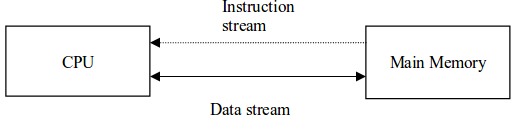
\includegraphics[scale=0.5]{1.png}
 \caption{Instruction and data stram}
 \label{fig:stream}
\end{figure}

La taxonomía de Flynn esta basado en cuantos flujos de datos e instrucciones existe en la máquina. Una máquina puede
tener un flujo simple o un flujo multiple de datos o instrucciones. Según como se convine estos dos tipos de flujo
se tiene una de las clasificaciones de Flynn (Figura \ref{fig:flynn}).

\begin{figure}
 \centering
 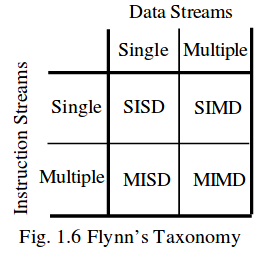
\includegraphics[scale=0.5]{2.png}
 \caption{Taxonomia de Flynn}
 \label{fig:flynn}
\end{figure}

\subsection{SISD}

Single Instruction stream and Single Data stream (SISD). En esta organización las instrucciones se ejecutan secuencialmente
en un sólo procesador sin explotar el paralelismo como las máquinas antiguas (DEC VAX, Apple Macintosh, CDC 7600, etc).
Esta confguración se muestra en la figura \ref{fig:sisd}

\begin{figure}
 \centering
 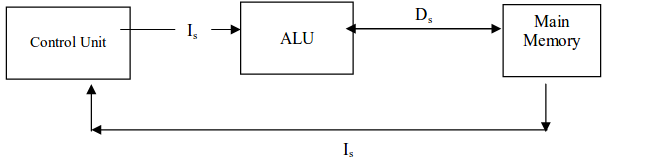
\includegraphics[scale=0.5]{3.png}
 \caption{Organización SISD}
 \label{fig:sisd}
\end{figure}

\subsection{SIMD}

Simple Instruction stream and Multiple Data Stream (SIMD). En esta organización varios elementos de procesamiento (PE)
trabajan bajo el control de una sola unidad de control. Todas las PEs reciven la misma instrucción  transmitida desde el CU.
La memoria principal puede ser dividida en modulos actuando como una memoria distribuida. Algunos ejemplos de esta
organización son  ILLIAC-IV, PEPE, BSP, STARAN, MPP y DAP. En la figura \ref{fig:simd} se muestra esta clasificación.

\begin{figure}
 \centering
 
\includegraphics[scale=0.5]{4.png}
 \caption{Organización SIMD}
 \label{fig:simd}
\end{figure}

\subsection{MISD}

Multiple Instruction stream and simple Data Stream (MISD). En esta organización varios elementos de procesamiento son
organizados por varias unidades de control. Cada unidad de control tiene su propio flujo de instrucciones hacia los 
respectivos PEs, pero todos los PEs procesan la información mediante un sólo flujo de datos, y se utiliza una memoria
compartida. El único ejemplo conocido el la C.mmp contruida por la universidad de Carnegie-Mellon. 
Esta clasificación es poco común debido al hecho de que la efectividad de los múltiples flujos de instrucciones
suele precisar de múltiples flujos de datos.
La configuración del MISD se muestra en la figura \ref{fig:misd}.

\begin{figure}
 \centering
 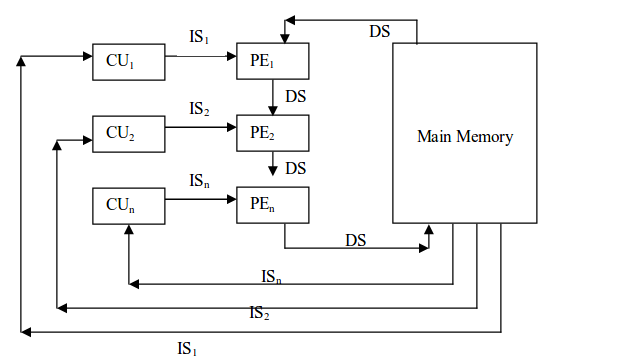
\includegraphics[scale=0.5]{5.png}
 \caption{Organización MISD}
 \label{fig:misd}
\end{figure}

\subsection{MIMD}

Las computadoras en la clase Mupltiple Instruction and Multiple Data Stream (MIMD) tiene varias unidades de control y
varios elementos de proceso, al igual que en el MISD, con la diferencia de que acá cada PE tiene su flujo de datos hacia
la memoria. Todos los sistemas multiprocesador funcionan bajo esta clasificación. En la figura \ref{fig:mimd} se detalla
esta organización.

\begin{figure}
 \centering
 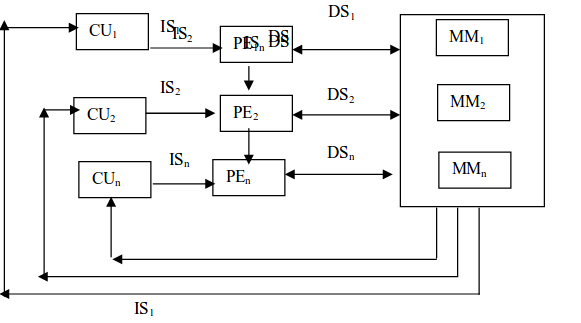
\includegraphics[scale=0.5]{6.png}
 \caption{Organización MIMD}
 \label{fig:mimd}
\end{figure}

\section{Redes de Interconexión}

Las redes de interconexion juegan un papel desicivo en el desempeño de los sistemas con memoria compartida y distribuida.

\subsection{Interconexiones de memoria compartida}

Los más utilizados son los buses y los crossbars. Los buses son cables de comunicación que permiten el acceso a la memoria.
La característica principal de un bus es que los cables de comunicación son compartidos con todos los dispositivos conectados.
Los buses son de bajo costo y flexibilidad; conectar un nuevo dispositivo tiene un costo muy bajo. Pero el problema radica al momento
de conectar varios dispositivos. Si aumentamos el número de procesadores conectados a un bus, baja la rapidez en que un procesador ingresa
a la memoria, ya que existe más posibilidad de que se quede esperando a otro. Los corssbars son una alternativa a los buses
que configura interruptores de tal manera que cada procesador tenga un módulo de memoria. Aunque som más rápidas que los buses, crear
los interruptores cuesta mucho.

\subsection{Interconexiones de memoria distribuida}

Las interconexiones de memoria distribuida se dividen en dos grupos: directas e indirectas. En una interconexión directa
cada interruptor esta conectado directamente con un procesador y con la memoria y los interruptores están conectados entre si.
El anillo y la tiroidal mesh son ejemplos de estas interconexiones. Estas dos son más rápidas que un bus por el número de conexiones,
permitiendo múltiples comunicaciones simultaneas. La tiroidal mesh son más costosas que los anillos, porque los interruptores
soportan cienco enlaces, mientras que en los anillos soportan sólo tres. \par

La banda de bisección es una medida para la conectividad de una interconexión. Para obtener esta medida se divide el sistema
en dos mitades con la misma cantidad de procesadores. La banda de bisección es el número de conecciónes que hay entre las
dos mitades. Para esto siempre se toma el pero caso, ya que se puede dividir un sistema de varias maneras.\\
El ancho de banda de un enlace es la velocidad a la que puede transmitir datos, y es muy utilizado para medir la calidad de la red. 
A menudo se mide en megabytes por segundo. Para obtenarel ancho de banda es muy similar a obtener la banda de bisección,
en vez de contar el número de enlaces entre las dos mitades, se suma el ancho de banda de dichas conecciones. \par

El hypercubo es una interconexión directa altamente conectada. Un hipercubo de dimensión uno se crea conectando dos
procesadores. Un hipercubo de dimensión dos se construye uniendo dos hipercubos de dimensión uno. Un hipercubo de
dimensión tres se contruye uniendo dos hipercubos de dimensión dos. Así se puede crear hipercubos de dimensión n. \par

En las interconexiones directas, los interruptores pueden no estar conectados directamente a un procesador. 
A menudo se muestran con enlaces unidireccionales y una colección de procesadores, cada uno de los cuales
tiene un enlace saliente y entrante, y una red de conmutación. La corssbar y la red omega son ejemplo simples de una
interconexión indirecta

\begin{thebibliography}{X}
  \bibitem{libro_2} \textsc{Eric Aubanel} \textit{Elements of Parallel Computing, December 6, 2016 by Chapman and Hall/CRC, pp 27-32}
 \bibitem{paper} \textsc{Daniel C. Hyde} \textit{Introduction to the Principles of Parallel Computation}
 \bibitem{libro} \textsc{Peter S. Pacheco.} \textit{An introduction to parallel programming, pp 29-42}
\end{thebibliography}



\end{document}
